%%%%%%%%%%%%%%%%%%%%%%%%%%%%%%%%%%%%%%%%%
% University/School Laboratory Report
% LaTeX Template
% Version 3.1 (25/3/14)
%
% This template has been downloaded from:
% http://www.LaTeXTemplates.com
%
% Original author:
% Linux and Unix Users Group at Virginia Tech Wiki 
% (https://vtluug.org/wiki/Example_LaTeX_chem_lab_report)
%
% License:
% CC BY-NC-SA 3.0 (http://creativecommons.org/licenses/by-nc-sa/3.0/)
%
%%%%%%%%%%%%%%%%%%%%%%%%%%%%%%%%%%%%%%%%%

%----------------------------------------------------------------------------------------
%	PACKAGES AND DOCUMENT CONFIGURATIONS
%----------------------------------------------------------------------------------------

%\documentclass{article}


\documentclass[12pt]{article}
%\documentclass[12pt]{book}

%\usepackage[version=3]{mhchem} % Package for chemical equation typesetting
%\usepackage[left=2.5cm,top=2.5cm,right=2.5cm,bottom=2.5cm]{geometry}
\usepackage[left=1.3cm,top=1.3cm,right=1.3cm,bottom=1.3cm]{geometry}
%\usepackage{siunitx} % Provides the \SI{}{} and \si{} command for typesetting SI units
\usepackage{graphicx,epstopdf} % Required for the inclusion of images
%\usepackage{graphicx} % Required for the inclusion of images
%\usepackage[outdir=./]{epstopdf}
%\epstopdfsetup{outdir=./}
\usepackage{blindtext}
%\usepackage[longnamesfirst]{natbib} % Required to change bibliography style to APA --> This produces NAT forces error with iteeer. Solution: Delete the option longnamesfirst and add the option numbers when loading the natbib package.
\usepackage[numbers,sort&compress]{natbib}
\usepackage{amsmath} % Required for some math elements 
%\setcitestyle{square}
%\usepackage{cite}
\usepackage{caption,setspace}
\usepackage{grffile}
\usepackage{enumerate}
%\usepackage[spanish,es-tabla]{babel}
%\usepackage[spanish]{babel}
\usepackage[british]{babel}
\usepackage[utf8]{inputenc}
\usepackage{amssymb}
%\usepackage{fourier} % Use the Adobe Utopia font for the document
\usepackage{datetime}                           % custom date
        \newdateformat{mydate}{\monthname[\THEMONTH] \THEYEAR}
%\usepackage{siunitx}
%\usepackage{sectsty}
%\allsectionsfont{\centering \normalfont\scshape}
\usepackage{subcaption}
\usepackage{courier}
\usepackage{enumitem}
\usepackage{textcomp}
\usepackage{multirow}
\usepackage[table,xcdraw]{xcolor}
\usepackage[version=3]{mhchem}
\usepackage{rotating}
\usepackage{subcaption}
\usepackage{mathtools}
\newcommand{\angstrom}{\mbox{\normalfont\AA}}
\usepackage{adjustbox}
\usepackage{lscape}
\usepackage{multicol}
\usepackage{textcomp}
%\usepackage{hyperref}
\usepackage{url}
\usepackage{enumitem}

%\usepackage{epstopdf}
%\usepackage[latin1]{inputenc}
%\usepackage[T1]{fontenc}
%POner para que el corte de palabras no lo corte donde le de la gana !!!
\setlength\parindent{0pt} % Removes all indentation from paragraphs
\captionsetup{font={footnotesize,sf,small,stretch=1},labelfont=bf}
%\captionsetup{font={footnotesize,sf,stretch=0.80},labelfont=bf}
\renewcommand{\labelenumi}{\alph{enumi}.} % Make numbering in the enumerate environment by letter rather than number (e.g. section 6)

\usepackage{afterpage}
\usepackage{rotating}
\usepackage{hhline}
\usepackage{fancyvrb}
\usepackage{floatpag}
\usepackage{amsthm}
\newtheorem{example}{Example}
\usepackage{empheq}
%\usepackage{grffile}
\newcommand*\widefbox[1]{\fbox{\hspace{2em}#1\hspace{2em}}}
%\usepackage{tikz}
\usepackage[makeroom]{cancel}
%\usetikzlibrary{decorations}
%\usetikzlibrary{decorations.pathreplacing}
%\usepackage{color,soul}
%\newcommand{\angstrom}{\text{\normalfont\AA}}
\usepackage{comment}
%\usepackage{subfig}
\usepackage{pdfpages} % To include pages of a pdf
%\usepackage{verbatim}
\usepackage{geometry}
%\usepackage[dvipsnames]{xcolor}

%\usepackage[most]{tcolorbox}
%\usepackage{tikz,lipsum,lmodern}
%\newtcolorbox{note}[1][]{%
%% enhanced jigsaw, % better frame drawing
%  colback=grey!5!white,
%% backgroundcolor=grey!40,%
%  borderline west={2pt}{0pt}{red}, % straigh vertical line at the left edge
%  sharp corners, % No rounded corners
%  boxrule=0pt, % no real frame,
%  fonttitle={\large\bfseries},
%  coltitle={black},  % Black colour for title
%  title={Note:\ },  % Fixed title
%% opacityfill=500,
%  opacityback=50,
%  attach title to upper, % Move the title into the box
%  #1
%}
\usepackage{titling}


\usepackage{tabularx}
%\newcommand\hb{HB}
\setlength{\parskip}{0em}

%\graphicspath{{/home/david/Trabajo/structures/RESULTADOS_NEW/CALCITE_I/115.015449/FREQCALC_on_SUPERCELL_Landau/SCANMODES_in_-20_20_0.4/Master_with_all_fitting_curves}}

\setlength{\droptitle}{-7em}   % This is your set screw

%\title{Calcite I - II phase transition  \vspace{-0.9cm}}%} % Title
\title{Common tangent procedure \vspace{-0.9cm}}%} % Title


%\author{David \textsc{Carrasco de Busturia}, Alessandro \textsc{Erba},\\ Giuseppe \textsc{Mallia} and Nicholas M. \textsc{Harrison}\vspace{-1cm} }
%\author{David \textsc{Carrasco de Busturia} and Nicholas M. \textsc{Harrison}} %\vspace{-1cm} }

%\author{David Carrasco de Busturia} % Author name
\date{\today} % Date for the report
%\date{}
%\mydate{\today}
%\date{\mydate}
%\date{\mydate\today}

%\begin{document}
\renewcommand\maketitlehookc{\vspace{-1.5ex}}
\begin{document}

\maketitle % Insert the title, author and date

\begin{comment}
\clearpage

%\chapter{Statement of the problem}



%\begin{comment}
\begin{table}[h!]
\centering
\begin{tabular}{|c|c|}
\hline
Volume     & Energy              \\ \hline
231.258240 & -3.766021868726E+03 \\ \hline
233.804750 & -3.766022502636E+03 \\ \hline
235.978198 & -3.766022676933E+03 \\ \hline
236.370909 & -3.766022674135E+03 \\ \hline
238.954760 & -3.766022411469E+03 \\ \hline
241.556358 & -3.766021721601E+03 \\ \hline
244.175148 & -3.766020622680E+03 \\ \hline
246.816007 & -3.766019128209E+03 \\ \hline
249.468797 & -3.766017256610E+03 \\ \hline
252.148054 & -3.766015013924E+03 \\ \hline
254.834741 & -3.766012425245E+03 \\ \hline
\end{tabular}
\caption{11 EOS volumes Aragonite: S.G. = $P m c n$}
\label{my-label}
\end{table}


\begin{sidewaystable}
\centering
\begin{adjustbox}{width={\textwidth},totalheight={\textheight},keepaspectratio}%
%\begin{table}[]
\begin{tabular}{ccclccccccccc}


\end{tabular}
\end{adjustbox}
  \caption{Scanmodes on Aragonite. In color the phases that I consider that are the same. }
    \label{phases}
\end{sidewaystable}
%\end{table}

\clearpage

\begin{figure}[h!]
\centering
\includegraphics[scale=0.9,clip]{/home/david/Trabajo/structures/SCANMODES/Aragonite_244_246_254_negative_modes/Aragonite_244_246_254.eps}
\caption{}
\label{diff_V_231_and_V_244}
\end{figure}



\RecustomVerbatimCommand{\VerbatimInput}{VerbatimInput}%
{fontsize=\footnotesize,
 %
 frame=lines,  % top and bottom rule only
 framesep=2em, % separation between frame and text
%rulecolor=\color{Gray},
 %
 label=\fbox{ Result de B III},
 labelposition=topline,
 %
 commandchars=\|\(\), % escape character and argument delimiters for
                      % commands within the verbatim
%commentchar=*        % comment character
}

\VerbatimInput{./freqs_only_negatives.txt}


\begin{verbatim}

Aragonite
EXTERNAL
OPTGEOM
END
END

\end{verbatim}

\begin{adjustbox}{width=\hsize, totalheight=\textheight, keepaspectratio}
\begin{BVerbatim}


A              B              C             ALPHA      BETA       GAMMA
5.84671408     8.04862162     5.01437439   90.000000  90.000000  90.001515
 1 T  20 CA   -2.600925756530E-01  4.151048814680E-01 -2.496387963369E-01
 3 T  20 CA   -2.399513667427E-01 -8.483484595548E-02  2.506049984881E-01
 5 T   6 C    -4.186005603935E-01 -2.378858814359E-01 -2.495795434709E-01
 7 T   6 C    -8.144642961300E-02  2.621340432766E-01  2.504687800166E-01
 9 T   8 O    -4.099183895024E-01 -7.825983482182E-02 -2.497931710868E-01
11 T   8 O    -9.009817249180E-02  4.217577078915E-01  2.506019750927E-01
13 T   8 O    -4.150537314122E-01 -3.192555582381E-01 -4.725896380099E-01
15 T   8 O    -8.505974813802E-02  1.809177587380E-01  2.730598196862E-02
17 T   8 O     8.499574017513E-02 -1.807874169360E-01 -2.649105352661E-02
19 T   8 O     4.150590412496E-01  3.190571898969E-01  4.736104668652E-01

\end{BVerbatim}
\end{adjustbox}

\end{comment}
\vspace{-3.5em}

\section{Introduction}

Given two energy-volume curves corresponding
to calcite I and II fitted to a cubic fit:

\begin{align}
f_{1} (x_1) &= a_{0} + a_{1} x_{1} + a_{2} x_{1}^{2} + a_{3} x_{1}^{3} \label{f1} \\
f_{2} (x_2) &= a_{4} + a_{5} x_{2} + a_{6} x_{1}^{2} + a_{7} x_{1}^{3} \label{f2}
\end{align}

Where the first dertivative is:

\begin{align}
f_{1}^{\prime} (x_1) = a_{1} + 2a_{2} x_{1} + 3a_{3} x_{1}^{2} \label{f1prime} \\
f_{2}^{\prime} (x_2) = a_{5} + 2a_{6} x_{2} + 3a_{7} x_{2}^{2} \label{f2prime} 
\end{align}

It is satisfied that $m$, the slope of the common tangent is:

\begin{equation}
\label{m}
m = \frac{f_{1} (x_1) - f_{2} (x_2)}{x_{1} - x_{2}} = f_{1}^{\prime} (x_1) = f_{2}^{\prime} (x_2) 
\end{equation}

We can write down a system of two equations:

\begin{comment}
\begin{equation}
\begin{cases}
\frac{f_{1} (x_1) - f_{2} (x_2)}{x_{1} - x_{2}} - f_{1}^{\prime} (x_1) = 0 \\
f_{1}^{\prime} (x_1) - f_{2}^{\prime} (x_2)  = 0 \label{eq:3}
\end{cases}
\end{equation}


\begin{equation}
  \left.\begin{aligned}
  a&=bbb\\
  c&=ddddddd\\
  e&=ffffff
\end{aligned}\right\} = stuff
\end{equation}

\begin{equation}
\left.\begin{aligned}
&\frac{f_{1} (x_1) - f_{2} (x_2)}{x_{1} - x_{2}} - f_{1}^{\prime} (x_1) = 0 \\
&f_{1}^{\prime} (x_1) - f_{2}^{\prime} (x_2)  = 0 \label{eq:3}
\end{aligned}\right\}
\end{equation}

\begin{equation}
\left\{
\begin{array}{ll}
\frac{f_{1} (x_1) - f_{2} (x_2)}{x_{1} - x_{2}} - f_{1}^{\prime} (x_1) &= 0 \\
f_{1}^{\prime} (x_1) - f_{2}^{\prime} (x_2)  &= 0 \label{eq:3}
\end{array}
\right.
\end{equation}



\begin{equation}
  \left\{
  \begin{array}{lcl}
    x_1 + x_2 + x_3 & = & 1 \\
    x_1 + x_2       & = & 2 \\
    x_1             & = & 3
  \end{array}
  \right.
\end{equation}

%\end{align}



\[
  \alpha(x)=\begin{cases}
               x\\
               \frac{1}{1+e^{-kx}}\\
               \frac{e^x-e^{-x}}{e^x+e^{-x}}
            \end{cases}
\]



\end{comment}


\begin{align}
\frac{f_{1} (x_1) - f_{2} (x_2)}{x_{1} - x_{2}} - f_{1}^{\prime} (x_1) &= 0 \label{eq1}\\
f_{1}^{\prime} (x_1) - f_{2}^{\prime} (x_2)  &= 0 \label{eq2}
\end{align}

The equation of the common tangent reads like:

\begin{align}
y - f_{1} (x_1)  &= m (x - x_1) \nonumber \\
\Aboxed{ y &= f_{1} (x_1) + m (x - x_1)} \label{common_tangent_eq}
\end{align}


\begin{figure}[h!]
\centering
  \begin{subfigure}[b]{0.4\textwidth}
    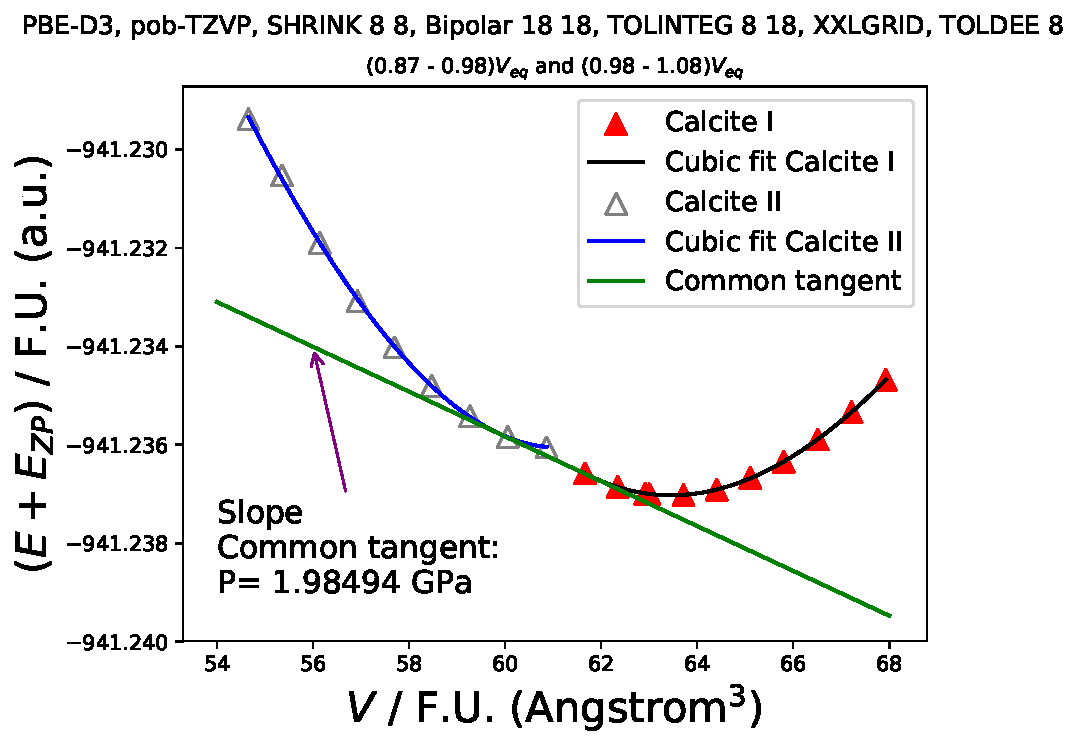
\includegraphics[width=\textwidth]{/home/david/Trabajo/structures/Scripts_on_Git_Hub/Common_Tangent/TEST/example_image/calcite_I_and_II_all_2_summary_better_plot.pdf}
    \caption{Picture 1}
    \label{fig:1}
  \end{subfigure}
\qquad
  %
  \begin{subfigure}[b]{0.4\textwidth}
    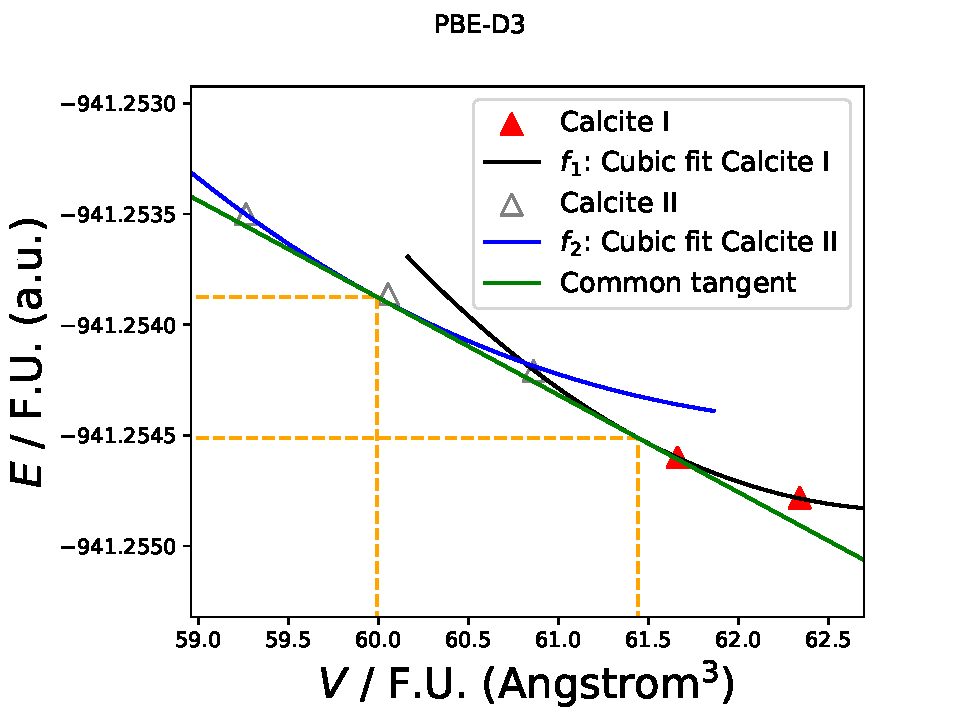
\includegraphics[width=\textwidth]{/home/david/Trabajo/structures/Scripts_on_Git_Hub/Common_Tangent/TEST/example_image/calcite_I_and_II_all_2_summary_better_plot_Zoomed.pdf}
    \caption{Picture 2}
    \label{fig:2}
  \end{subfigure}
\end{figure}


Because $f_{1}(x_1)$ and $f_{2} (x_2)$
depend only on $x_1$ and $x_2$,
the system of equations based on Eqns (\ref{eq1}) and (\ref{eq2}),
contain two unknowns, $x_1$
and $x_2$.
Once obtained $x_1$ and $x_2$,
$m$ can be obtained as Eq. \ref{m}.
Once reached this point,
we can then go to Eq. \ref{common_tangent_eq} and sort out the common tangent equation

%\bibliographystyle{ieeetr}
\bibliographystyle{IEEEtran}
\bibliography{/home/david/Dropbox/Bibliography-David/library}


\end{document}
%

